\subsection{Matching based solutions} 

Some versions of $\Problem$ boil down to matching problems. These are in 
particular problems related to replica seletion, e.g. the basic version of 
$\Problem$: each VM 
is allready placed, the loactions of all chunks are known, and we have to 
compute an assignment (or matching) of VMs to chunks, such that each VM is 
assigned to 
exactly one chunk, and each chunk is assigned to exactly one chunk. Hence we 
can transform each instance of the basic $\Problem$ to a minimum weight 
perfect bipartite 
matching problem\cite{schrijver_combinatorial_optimization}. One of the sets 
is formed by $\VirtualNodes$, the other by the 
set of chunks. A VM has an edge to each chunk. The costs of these edges are 
defined by the hop count between the VM and the chunk in the host graph. Each 
edge which is chosen for the solution of the matching problem, indicates that 
the chunk is assigned to the vm of the edge.

\begin{figure}
\begin{minipage}[b]{0.49\linewidth}
\centering
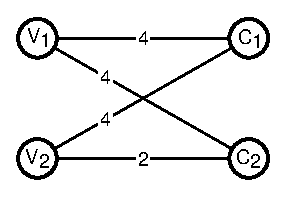
\includegraphics[width =\columnwidth]{figs/matching_basic} 
\caption{The matching problem generated from the basic scenario in 
Figure~\ref{fig:basic_problem}}
\label{fig:matching_basic}
\end{minipage}
\quad
\begin{minipage}[b]{0.49\linewidth}
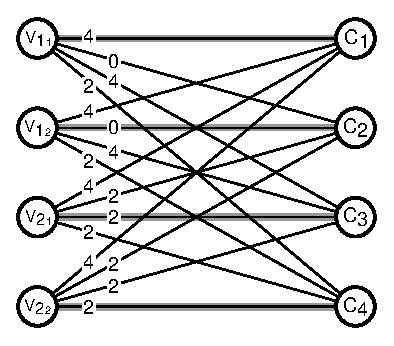
\includegraphics[width = \columnwidth]{figs/matching} 
\caption{The matching problem for the instance from 
Figure~\ref{fig:model_combined} without $cv$. The solution is indicated by 
shadowed lines.}
\label{fig:matching}
\end{minipage}
\end{figure}

Figure~\ref{fig:matching_basic} shows an example of this for the instance from 
Figure~\ref{fig:basic_problem}: $\NodeMapping(\VirtualNode_1)$ is four hops 
away from all chunks - in the matching problem, this is depicted by the edge 
weight on the edges, from $\VirtualNode_1$. $\NodeMapping(\VirtualNode_2)$ is 
two hops away from $\Chunk_2$, and 4 hops away from $\Chunk_1$. Hence the 
weight of the edge $(\NodeMapping(\VirtualNode_2),\Chunk_2)$ is $2$, while the 
weight on the edge to $\Chunk_1$ is $4$. The solution to the minimum weight 
perfect bipartite matching contains the edges $(\NodeMapping(\VirtualNode_1), 
\Chunk_1)$ and $(\NodeMapping(\VirtualNode_2), 
\Chunk_2)$, which is excatly the Chunk to VM assignment $\VmChunkAssignment$ 
which we identified as an optimal solution in Section~\carlo{TODO}.


This approach can also be used to solve instance of $\Problem$, which have the 
$ma$ or $r$ property - or even both. 
To Account for the $ma$ property, a single VM has to process exactly 
$\MaFactor$ VMs. Hence we can clone a VM to be represented by $\MaFactor$ Nodes.
In order to incorporate the different 
replicas of the chunks, we depict all copies of a given $\ChunkTypes$ in a 
single %$\ChunkType$ 
node. We connect each VM to all $\ChunkTypes$ using the 
lowest hop count to one of the copies as the weight.

Figure~\ref{fig:matching} illustrates this for the scenario from 
Figure~\ref{fig:model_combined} without the $cv$ property: The $2$ VMs are 
cloned into $\MaFactor = 2$ VMs each - resulting in a total of $4$ VM nodes in 
the matching problem. The $\RedundancyFactor = 2$ chunks of each chunk type are 
aggreated $\Chunk_j$ into a single chunk type node in the matching problem - 
resulting in a total of $4$ chunk type nodes in the matching graph. The weight 
on the edges between all clones of a specific VM and a chunk type are set to 
the minimum distance. This can for instance be observed at the egdes connecting 
the two clones of $\VirtualNode_1$ to $\Chunk_2$: both weights are 0.



Many algorithms solve the minimum weith perfect matching problem on bipartite 
graphs. The algorithms runtimes depend on  the number of nodes in the 
graph $n$, the number of edges in the graph $m$, and the largest magnitude of 
an edge weight $N$. An efficient algorithm is described by Gabow et al. in 
\cite{gabow_scaling_algorithm} and provides a runtime of $\mathcal{O}(n^{3/4} 
\cdot m \cdot \log N)$ which translates to $\mathcal{O}((\MaFactor \cdot \Vms + 
\ChunkTypes)^{3/4} \cdot  \MaFactor \cdot \Vms \cdot \ChunkTypes \cdot \log 
(2 \cdot h(\Tree)))$, where $h(T)$ denotes the height of the tree.